% !TeX root = ../index.tex

\section{Einleitung}\label{sec:einleitung}

Dieser Bericht beschreibt eine Laborarbeit, welche im Rahmen der Vorlesung \enquote{W3M20018.1 Data Science \& Big Data} durchgeführt wurde.\footnote{\href{https://farberg.de/talks/big-data/?01\%20-\%20Introduction.md\#/2}{https://farberg.de/talks/big-data/?01 - Introduction.md\#/2}}
Gegenstand der Laborarbeit ist die Abwandlung eines vorgegebenen Big Data Setups, um damit einen eigens ausgewählten Use Case abzubilden.\footnote{\href{https://farberg.de/talks/big-data/?06\%20-\%20Use\%20Case.md\#/}{https://farberg.de/talks/big-data/?06 - Use Case.md\#/}}
Die praktischen Ergebnisse der Arbeit sind im GitHub Repository \href{https://github.com/kevinsieverding/dhbw-w3m200181-app}{kevinsieverding/dhbw-w3m200181-app} zu finden.

Im Folgenden beschreiben Abschnitt \ref{sec:use-case} den gewählten Use Case und Abschnitt \ref{sec:architektur} die gewählte Architektur und Umsetzung.
Daraufhin legt Abschnitt \ref{sec:funktion} die genaue Funktion der Anwendung im Detail dar.
Abschnitt \ref{sec:fazit} legt abschließend ein Fazit dar.

\section{Use Case}\label{sec:use-case}

Das originale Setup stellt eine Reihe von Artikeln über einen Web-Server bereit, zeichnet Seitenaufrufe auf und schreibt sie in Kafka, von wo sie ein Spark Job aufnimmt und aggregiert, um Popularitätsstatistiken zu erstellen, welche wiederum auf der Web-Seite angezeigt werden.
Der Use Case befasst sich also mit einer simplen Analyse von Nutzerverhalten.

\subsection{Brainstorming}

Um einen geeigneten Use Case zu wählen, habe ich zunächst ein Brainstorming betrieben, bis ich eine zufriedenstellende Idee entwickelt hatte.
Im Folgenden möchte ich einige meiner verworfenen Ideen vorstellen, bevor ich den von mir letztendlich gewählten Use Case näher beschreibe.

\subsubsection{Warenkorbanalyse mittels Apriori Algorithmus}

Mein erster Gedanke war, in bei der Nutzeranalyse zu bleiben und eine andere Form der Analyse zu implementieren.
Da ich in meiner Arbeit als Entwickler bei der SAP im Bereich Standardsoftware für den Einkauf mit internen Bestellplatformen zu tun habe, überlegte ich eine simple Warenkorbanalyse mittels des \enquote{Apriori} Algorithmus zu implementieren.
\parencite{agrawal_fast_1994}

Hierzu würde ich einen simplen Web-Shop implementieren, welcher dem Nutzer einen Katalog von Produkten anzeigt, welche dieser in seinen Warenkorb legen und bestellen kann.
Die Bestellungen mitsamt der Positionen würden in Kafka geschrieben werden, wo ein Spark Job den Apriori Algorithmus anwendet, um Tupel von häufig zusammen gekauften Produkten zu identifizieren.
Diese Information würde der Spark Job in eine MariaDB Datenbank persistieren, wo sie von der Web-App abgefragt werden könnte, um dem Nutzer einen Vorschlag wie \enquote{Kunden kauften ebenfalls:  \ldots} anzuzeigen, wie man ihn von den Webseiten von vielen großen Online-Händlern kennt.

Letzenendes habe ich mich dagegen entschieden diesen Use Case so zu implementieren, weil mir der notwendige Aufwand als schwierig abzuschätzen und tendenziell groß erschien.
Die Implementierung des Web-Shops mit nicht-existenten Kenntnissen in der Web-Entwicklung, sowie die nicht trivial erscheinende Implementierung des Apriori Algorithmus in Spark waren dabei ausschlaggebend.
Aus diesem Grund habe ich mich nach einem Use Case umgeschaut, welcher in einem kleineren Rahmen umzusetzen sei.

\subsubsection{Analyse der Parksituation in Heidelberg}

Anschließend überlegte ich die Parksituation in meiner aktuellen Heimatstadt Heidelberg zu analysieren.
Die größte Herausforderung dabei schien mir, geeignete Daten zu finden.
Unter \url{https://parken.heidelberg.de/} bietet die Stadt Heidelberg bereits eine digitale Übersicht der aktuellen Parksituation an, woraus sich schließen lässt, dass diese Daten nicht nur bereits gesammelt und analysiert werden, sondern auch über das Internet zugreifbar sind.

Leider stellte sich bei einer oberflächlichen Analyse der Webseite heraus, dass die zugrundeliegende Daten-API nicht ohne Weiteres über andere Wege zugreifbar ist.
Während sich mit hoher Wahrscheinlichkeit ein Weg finden ließe, die API dennoch programmatisch auszulesen, so wollte ich die damit einhergehende Unsicherheit und den möglichen Aufwand für das Schreiben eines Clients/Crawlers für die API vermeiden.
Daher habe ich auch diese Option verworfen.

\subsection{Analyse von Messwerten zur Überwachung von Industriemaschinen}

Als drittes habe ich mich mit einem weiteren Umfeld auseinandergesetzt, in dem Big Data seit längerem eine große Rolle spielt: Predictive Maintenance.
\citeauthor{hashemian_state---art_2011} beschreibt moderne Predictive Maintenance wie folgt: \enquote{[A]utomated methods that use advanced signal processing techniques based on pattern recognition, including neural networks, fuzzy logic, and data-driven empirical and physical modeling.} \parencite{hashemian_state---art_2011}

Hier ließen sich verschiedene frei verfügbare Datensätze finden, welche als Basis für die Implementierung einer Big Data Anwendung dienen konnten.
Ich bin schließlich auf einen Datensatz der ZeMA gGmbH gestoßen, welcher im Rahmen von \cite{helwig_condition_2015} erstellt wurde und Daten von verschiedenen Sensoren eines hydraulischen Test-Systems enthält, die über mehrere Betriebszyklen hinweg aufgezeichnet wurden.\footnote{\url{https://archive.ics.uci.edu/ml/datasets/Condition+monitoring+of+hydraulic+systems}}

\begin{figure}[H]
  \centering
  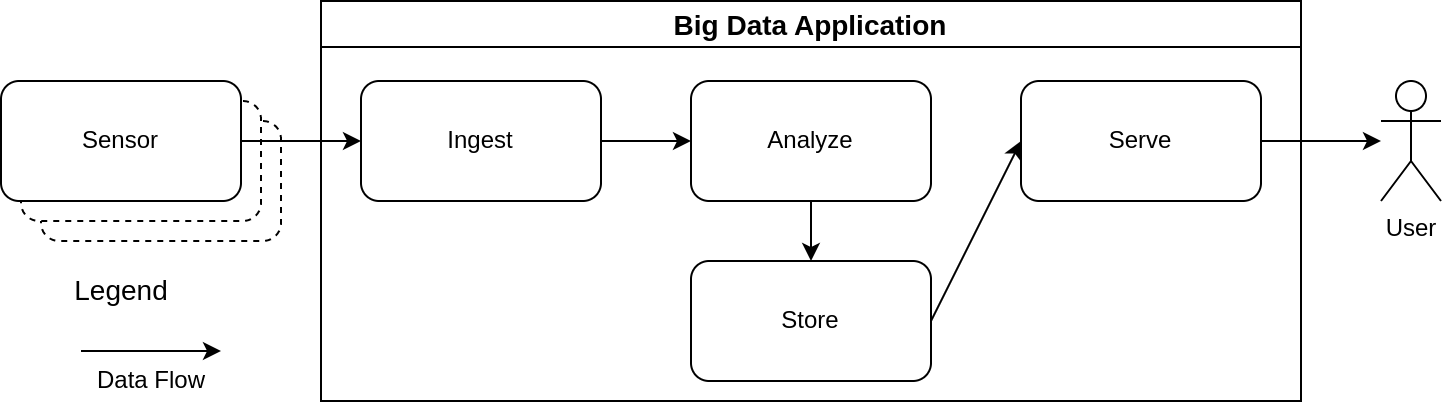
\includegraphics[width=0.9\textwidth]{use-case.drawio.png}
  \caption{Grobes Modell des gewählten Use Case}\label{fig:use-case}
\end{figure}

Auf Basis dieses Datensatzes definierte ich den Use Case, für den ich das Big Data Setup aufbauen wollte.
Abbildung \ref{fig:use-case} zeigt, wie zunächst Messwerte von einem oder mehreren Sensoren in die Applikation geladen werden sollen.
Diese Daten sollen analysiert und die erarbeiten Ergebnisse persistiert werden.
Persistierte Ergebnisse können anschließend Nutzern zur Verfügung gestellt werden.

\section{Architektur}\label{sec:architektur}

Da gemäß der Aufgabenstellung die existierende Anwendung angepasst werden sollte, und diese bereits der Kappa-Architektur folgt, so tut dies auch die von mir gestaltete Anwendung.
Ohnehin erscheint mir für den gewählten Use Case die Kappa-Architektur sinnvoller als die Lambda-Architektur, da getrennte Batch und Speed Layer die Anwendung unnötig verkomplizieren würden.

Abbildung \ref{fig:architektur} zeigt die Architektur der implementierten Big Data Anwendung und eine vereinfachte Darstellung des Datenflusses zwischen den Komponenten, um ihr Zusammenspiel abzubilden.
Der Big Data Stack ist im Hinblick auf die verwendeten Produkte identisch mit der vorgegebenen Anwendung.
Apache Kafka dient als Streaming Plattform, während ein Apache Hadoop Cluster mitsamt YARN ein HDFS als Data Lake und Apache Spark als Stream Processor bereitstellt.

\begin{figure}[H]
  \centering
  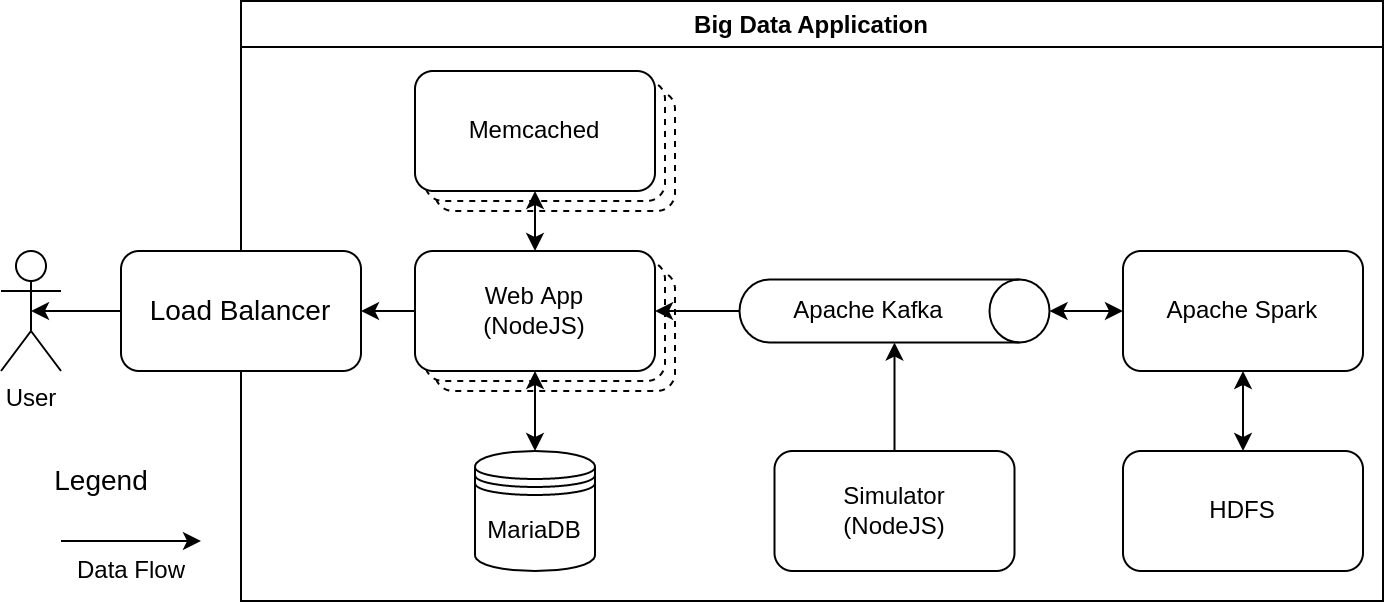
\includegraphics[width=0.9\textwidth]{architecture.drawio.png}
  \caption{Architektur der implementierten Big Data Anwendung}\label{fig:architektur}
\end{figure}

Im proprietären Teil der Anwendung finden sich mehrere Instanzen eine NodeJS Web-App, welche Nutzern eine API bereitstellt.
Diese App verwendet einen Memcached als Soft State zur, um Ergebnisse von Datenbankabfragen für kurze Zeit zu zwischenzuspeichern und somit selbst bei hoher Last Anfragen mit niedrigen Latenzen bearbeiten zu können.
Zur Persistenz nutzt die App eine MariaDB Instanz.
Diese wird---im Kontrast mit der ursprünglichen Anwendung---exklusiv von der Web-App verwendet und nicht ebenfalls von der Spark Anwendung.

Anstatt sowohl die Web-App als auch Spark an die Datenbank zu koppeln, schreibt Spark die Ergebnisse seiner Analysen in Kafka zurück.
Diese Nachrichten werden von der Web-App konsumiert und in die Datenbank geschrieben.
Dadurch sind die Komponenten nur gegen Kafka gekoppelt und die Datenhaltung der Web-App stellt nur ein materialisiertes Abbild der Daten in Kafka dar, welches zum Beispiel nach einem Ausfall, oder nach Beheben eines Programmfehlers, einfach weggeworfen und neu gebildet werden kann.

Wie auch in der ursprünglichen Anwendung, werden alle Teil-Komponenten dieser Anwendung in einem Kubernetes Cluster bereitgestellt.
Dieses stellt zudem den Load Balancer, welcher die Web-App für Nutzer zugreifbar macht, und die Anfragen über die verschiedenen Instanzen der App verteilt.

Als letzte zu nennende Komponente stellt der Simulator ebenfalls eine Abkehr von dem Modell des Use Case in Abbildung \ref{fig:use-case} dar.
Um Sensordaten in die Big Data Anwendung zu bringen, sieht der Use Case eine dedizierte Komponente vor.
Konkret könnte dies ein MQTT-Gateway sein, das es MQTT-Clients erlaubt Nachrichten mit Messwerten über das bei IoT-Devices beliebte Protokoll an die Anwendung zu senden.
Diese Nachrichten könnten dann in den Kafka gespeist und von Spark verarbeitet werden.

Im Laufe der Laborarbeit habe ich mich jedoch zunächst für einen pragmatischeren Ansatz entschieden.
Nämlich, eine Komponente einzubauen, welche ein solches Gateway simuliert, indem es Nachrichten mit pseudo-zufälligen Werten in Kafka schreibt.

\section{Funktion}\label{sec:funktion}

Konkret generiert der Simulator im Sekundentakt Temperaturwerte zwischen 30~°C und 80~°C---in Anlehnung an den Datensatz von \cite{helwig_condition_2015}.
Damit diese Werte nicht zu unrealistisch sind, werden sie im Wertebereich normalverteilt generiert.
Die App schreibt die Werte im JSON Format auf das Kafka Topic \path{de.kevinsieverding.supervizor.temperature}.
Das Listing \ref{lst:temperature-message} zeigt ein Beispiel für den Inhalt einer solchen Nachricht.

\begin{listing}[H]
  \inputminted{json}{assets/src/temperature-message.json}
  \caption{Beispielinhalt einer Kafka-Nachricht mit generiertem Temperaturwert}\label{lst:temperature-message}
\end{listing}

Diese Nachrichten werden von Spark aufgegriffen und mittels Microbatching in 30 Sekunden langen, rollenden Zeitfenstern verarbeitet.
Bei der Verarbeitung werden die Werte in die Zeitfenster gruppiert und nur der maximale Temperaturwert innerhalb des Fensters behalten.
Liegt dieser Wert über dem Grenzwert von 66 °C, so schreibt Spark eine Nachricht auf das Topic \path{de.kevinsieverding.supervizor.temperature-warnings}.
Diese enthält die Start- und End-Zeitpunkte des Zeitfensters, sowie den Temperaturwert.
Das Listing \ref{lst:temperature-warning-message} zeigt ein Beispiel für den Inhalt einer solchen Nachricht.

\begin{listing}[H]
  \inputminted{json}{assets/src/temperature-warning-message.json}
  \caption{Beispielinhalt einer Kafka-Nachricht mit Warnung vor zu hohem Temperaturwert}\label{lst:temperature-warning-message}
\end{listing}

Diese Nachrichten mit Warnungen über Messwerte, welche die bestimmten Grenzwerte überschreiten, werden wiederum von der Web-App konsumiert und in der Datenbank persistiert.
Über den API-Endpunkt \path{/warnings} können alle gespeicherten Warnungen abgefragt werden, während der Endpunkt \path{/warnings/:id} es erlaubt eine bestimmte Warnung über ihre ID abzufragen.
Die Ergebnisse der dafür notwendigen Datenbankabfragen werden in den Memcached Instanzen für fünf Sekunden zwischengespeichert.

\section{Fazit}\label{sec:fazit}

Die vorgestellte Laborarbeit wandelt die gegebene Anwendung gemäß der Aufgabenstellung ab, um einen unteschiedlichen Big Data Use Case zu implementieren.
Hierbei widmet sich die entwickelte Anwendung der Analyse von Messwerten von simulierten Temperatursensoren.
Die Analyse beschränkt sich darauf zu prüfen ob die Messwerte einen festen Grenzwert überschreiten.
Ist dies der Fall, wird diese Information über Kafka an eine Web-App kommuniziert, welche diese persistiert und über eine API bereitstellt.
Im Gegensatz zu der ursprünglichen Anwendung, wird die Datenbank exklusiv von der Web-App verwendet.
Die Spark und Web Apps integrieren ausschließlich über Kafka.

Es präsentieren sich zwei offensichtliche Möglichkeiten zur Weiterentwicklung.
Erstens, könnte die Simulator App durch ein MQTT Gateway ersetzt werden, wodurch die Architektur den Anforderungen eines realistischeren Form des Use Case besser gerecht werden könnte.
Zur Veranschaulichung der Funktionalität, könnten schlanke MQTT Clients entwickelt werden, die anstatt Werte zu generieren, Werte aus dem Datensatz von \cite{helwig_condition_2015} über das Gateway in die Anwendung spielen.

Zweitens, ist die Analyse in Spark in der vorliegenden Form wenig \textit{predictive}.
Um dem Anspruch von Predictive Maintenance näher zu kommen, könnten womöglich Funktionen der SparkML Bibliothek verwendet werden, um anhand der Sensorwerte die verbleibende Nutzdauer der Maschine vorherzusagen.
